
\documentclass[journal,transmag]{IEEEtran}
\hyphenation{op-tical net-works semi-conduc-tor}

\usepackage{enumitem}

\usepackage{amsmath}


% *** GRAPHICS RELATED PACKAGES ***
%
\ifCLASSINFOpdf
   \usepackage[pdftex]{graphicx}
  % declare the path(s) where your graphic files are
  % \graphicspath{{../pdf/}{../jpeg/}}
  % and their extensions so you won't have to specify these with
  % every instance of \includegraphics
  % \DeclareGraphicsExtensions{.pdf,.jpeg,.png}
\else
  % or other class option (dvipsone, dvipdf, if not using dvips). graphicx
  % will default to the driver specified in the system graphics.cfg if no
  % driver is specified.
  % \usepackage[dvips]{graphicx}
  % declare the path(s) where your graphic files are
  % \graphicspath{{../eps/}}
  % and their extensions so you won't have to specify these with
  % every instance of \includegraphics
  % \DeclareGraphicsExtensions{.eps}
\fi
% graphicx was written by David Carlisle and Sebastian Rahtz. It is
% required if you want graphics, photos, etc. graphicx.sty is already
% installed on most LaTeX systems. The latest version and documentation
% can be obtained at: 
% http://www.ctan.org/pkg/graphicx
% Another good source of documentation is "Using Imported Graphics in
% LaTeX2e" by Keith Reckdahl which can be found at:
% http://www.ctan.org/pkg/epslatex
%
% latex, and pdflatex in dvi mode, support graphics in encapsulated
% postscript (.eps) format. pdflatex in pdf mode supports graphics
% in .pdf, .jpeg, .png and .mps (metapost) formats. Users should ensure
% that all non-photo figures use a vector format (.eps, .pdf, .mps) and
% not a bitmapped formats (.jpeg, .png). The IEEE frowns on bitmapped formats
% which can result in "jaggedy"/blurry rendering of lines and letters as
% well as large increases in file sizes.
%
% You can find documentation about the pdfTeX application at:
% http://www.tug.org/applications/pdftex






\begin{document}

\title{\textsc{Análisis de Características del Suelo para la Clasificación de Cultivos Agrícolas}}

\author{
\IEEEauthorblockN{William Andrés Gómez Roa}
\IEEEauthorblockA{Pontificia Universidad Javeriana, Bogotá, Colombia}
\IEEEauthorblockA{Inteligencia Artificial - Proyecto Final}


}
% The paper headers
\markboth{Clusters del Cacao}%
{Shell \MakeLowercase{\textit{et al.}}: Bare Demo of IEEEtran.cls for IEEE Transactions on Magnetics Journals}
\IEEEtitleabstractindextext{%

	\begin{abstract}
In this project, we conducted a comprehensive analysis of soil properties and absorbance at different wavelengths to classify agricultural crops. Unsupervised learning techniques were employed, and a binary classifier was applied to determine the cluster to which the cocoa crop belongs.
	\end{abstract}
	\begin{IEEEkeywords}
SoilProperties, UnsupervisedLearning, ClusterAnalysis, MachineLearning, AgriculturalCrops, Absorbance, Fertilizer.
	 	\end{IEEEkeywords}}

\maketitle
\IEEEdisplaynontitleabstractindextext
\IEEEpeerreviewmaketitle

\section{INTRODUCCIÓN}
En este proyecto, se realizó un análisis exhaustivo de los datos de propiedades del suelo y se aplicaron técnicas de aprendizaje automático. Se exploraron diferentes algoritmos supervisados y no supervisado, como el algoritmo K-means, para identificar patrones y agrupar los datos en diferentes categorías. Además, se implementaron clasificadores binarios utilizando para determinar a que clúster pertenecen los cultivos de cacao. Se evaluaron diversas métricas de desempeño para medir la calidad de los modelos y se realizaron análisis estadísticos para examinar las relaciones entre las variables del suelo y los cultivos.

\section{DESARROLLO}

Durante el desarrollo del proyecto, se realizó una exploración y limpieza exhaustiva de los datos, incluyendo la imputación de valores faltantes y la escalización de los datos. A continuación, se aplicó el análisis de componentes principales (PCA) para reducir la dimensionalidad y seleccionar las variables de interés relacionadas con las propiedades del suelo y la radiación.Posteriormente, se implementó el algoritmo de K-means para identificar clústeres basados en las características seleccionadas. Utilizando el método del codo y el coeficiente de silueta, para determinar el número óptimo de clústeres. Luego, se realizó una clasificación binaria utilizando algoritmos como regresión logística, SVM y árboles de decisión para asignar los cultivos agrícolas a los clústeres identificados, centrándonos específicamente en el cultivo de cacao. Por último, se evaluó el modelo utilizando conjuntos de entrenamiento, validación y pruebas, validación cruzada y se utilizaron métricas como precisión, coeficiente de correlación de Matthews (MCC) y la matriz de confusión para evaluar el rendimiento del modelo de clasificación. No fue necesario aplicar regularización.
El proyecto se realizó en un ‘jupyter notebook’ y se subió a Github junto con el dataset, los objetivos iniciales del proyecto y un video explicativo del mismo.
  

\section{RESULTADOS } 
\subsection{Agruapamiento por Clusters utilizando k-means}
Se utilizaron los datos de pH, Al, Mg, Mn y los demás minerales del suelo junto con la Absorbancia para dividir el dataset en 2 clusters. Luego se observó la distribución de los cultivos de 'CACAO' en dichos clusters como se observa a continuación.
\begin{figure}[!h]
    \center
    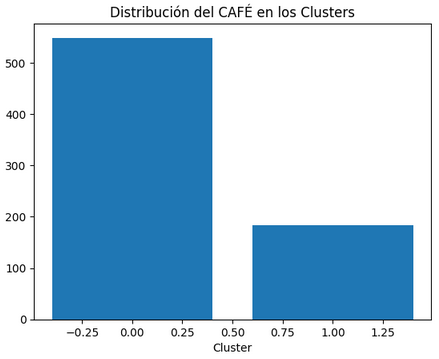
\includegraphics[width=7cm]{imgs/s1.png}
    \caption{Distribución de los cultivos de Cacao en los 2 clusters encontrados}
    \label{1}
\end{figure}

Así mismo se realizó la clasificiación supervisada de los cultivos de cacao en los 2 clusters previamente mencionados y se evaluaron las métricas que se observana continuación.

\begin{figure}[!h]
    \center
    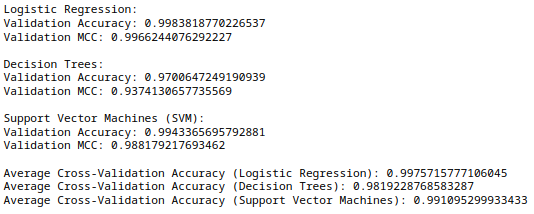
\includegraphics[width=8cm]{imgs/s2.png}
    \caption{Métricas de los clasificadores binarios entrenados}
    \label{1}
\end{figure}

Todo se realizó en Jupyter-Notebook

%%%%%%%%%%%%%%%%%%%%%%%%%%%%%%%%%%%%%%%%%%%%%%%%%%%%RESULTADOS


\section{Conclusion}
Finalmente, hemos concluido con el desarrollo del proyecto final de IA despues de analizar un dataset real sobre las propiedades del suelo y la absorbancia en diferentes longitudes de onda.

Mi idea inicial era entender los Fertiliantes que se aplican a los suelos, es decir yo quería analizar como las caracteristicas de pH, Al, Fe, Mg, Mn, Cu, B, y demas minerales influyen en la caracterización del suelo guiada por el tipo de cultivo y por la ubicación geogŕafica (Departamento). Es por esto que el análisis inicial realizado con aprendizaje No Supervisado con el algorirmo K-means utilizo las caracteristicas de interes antes mencionadas junto con la radiación de los diferentes longitudes de onda. El proyecto concluyo estudiando el comportamiento de los 2 clsuters que se generaron tras la busqueda. Se intentó explorar un poco los datos y ver relaciones intrinsecas de los clusteres. Finalmente se decidío realizar un clasificado binario con el fin de determinar para un tipo de cultivo específico que fue 'CACAO' a que cluster de los hallados previamente pertenecian.

Esto puede servir para comprender las caracteristicas del suelo que se relacionen con un cluster en particular y por eso identificar a que tipo de cluster pertenecen los cultivos es de gran utilidad para indagar y conocer más sobre las propiedades adecuadas de los suelos.



\appendices




\ifCLASSOPTIONcaptionsoff
  \newpage
\fi




\end{document}
